% Gerado por analysis/artigo2.py: menções (N1) x adoção externa (N3)
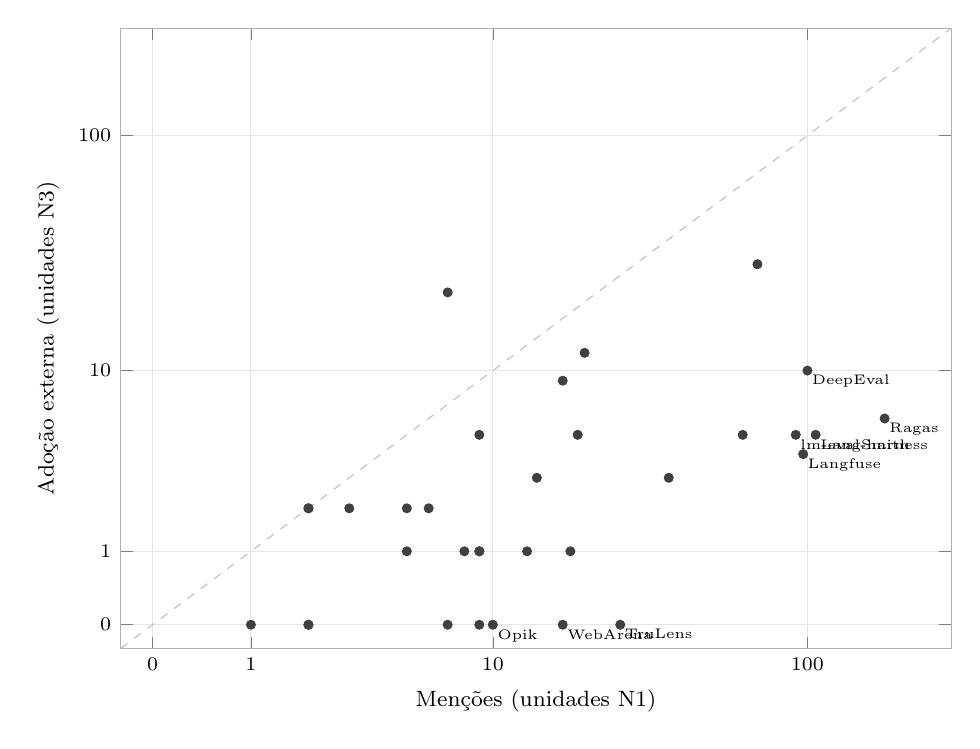
\begin{tikzpicture}
  \begin{axis}[width=\columnwidth, height=0.78\columnwidth,
      xmode=log, ymode=log,
      xmin=0.8, ymin=0.8, xmax=278, ymax=278,
      xtick={1,2,11,101}, xticklabels={0,1,10,100},
      ytick={1,2,11,101}, yticklabels={0,1,10,100},
      xlabel={Menções (unidades N1)}, ylabel={Adoção externa (unidades N3)},
      label style={font=\footnotesize}, tick label style={font=\scriptsize},
      grid=major, major grid style={gray!20}, axis line style={gray!60}]
    \addplot[gray!50, dashed, domain=0.8:278, samples=2] {x};
    \addplot[only marks, mark=*, mark size=1.6pt, black!75]
      coordinates {(71,30) (8,23) (21,13) (101,11) (18,10) (174,7) (107,6) (93,6) (64,6) (20,6) (10,6) (98,5) (38,4) (15,4) (6,3) (7,3) (4,3) (3,3) (3,3) (14,2) (10,2) (9,2) (10,2) (6,2) (19,2) (11,1) (27,1) (18,1) (2,1) (3,1) (3,1) (10,1) (8,1)};
    \node[anchor=north west, font=\tiny, inner sep=1.5pt] at (axis cs:174,7) {Ragas};
    \node[anchor=north west, font=\tiny, inner sep=1.5pt] at (axis cs:107,6) {LangSmith};
    \node[anchor=north west, font=\tiny, inner sep=1.5pt] at (axis cs:101,11) {DeepEval};
    \node[anchor=north west, font=\tiny, inner sep=1.5pt] at (axis cs:98,5) {Langfuse};
    \node[anchor=north west, font=\tiny, inner sep=1.5pt] at (axis cs:27,1) {TruLens};
    \node[anchor=north west, font=\tiny, inner sep=1.5pt] at (axis cs:18,1) {WebArena};
    \node[anchor=north west, font=\tiny, inner sep=1.5pt] at (axis cs:93,6) {lm-eval-harness};
    \node[anchor=north west, font=\tiny, inner sep=1.5pt] at (axis cs:11,1) {Opik};
  \end{axis}
\end{tikzpicture}
